\documentclass{beamer}
\usetheme{Boadilla}

\title{Plant Seedlings Classification}
\subtitle{Using Instagram and ImageNet pretrained deep convolutional networks for seedling species image classification}
\author{Julian Cabezas Pena}
\institute{a1785086}
\date{\today}

\begin{document}
	
\begin{frame}
	\titlepage
\end{frame}	


\begin{frame}
	\frametitle{Introduction}
	
	\begin{itemize}
		\item Image Classification field is dominated by deep convolutional networks
		\item Problem: Long time to train
		\item One Solution: Pretrained models using Imagenet and Instagram
		\item Application of pretrained model for Plant Seedling Kaggle competition
	\end{itemize}
	
\end{frame}

\begin{frame}
	
	\frametitle{Data preprocessing}
	
	\begin{itemize}
		\item 12 weed and crop species 
		\item The train data contains 4750 annotated species (25\% as validation data)
		\item Test data: 794 unannotated images
		
		\begin{figure}[h]
			\begin{center}
				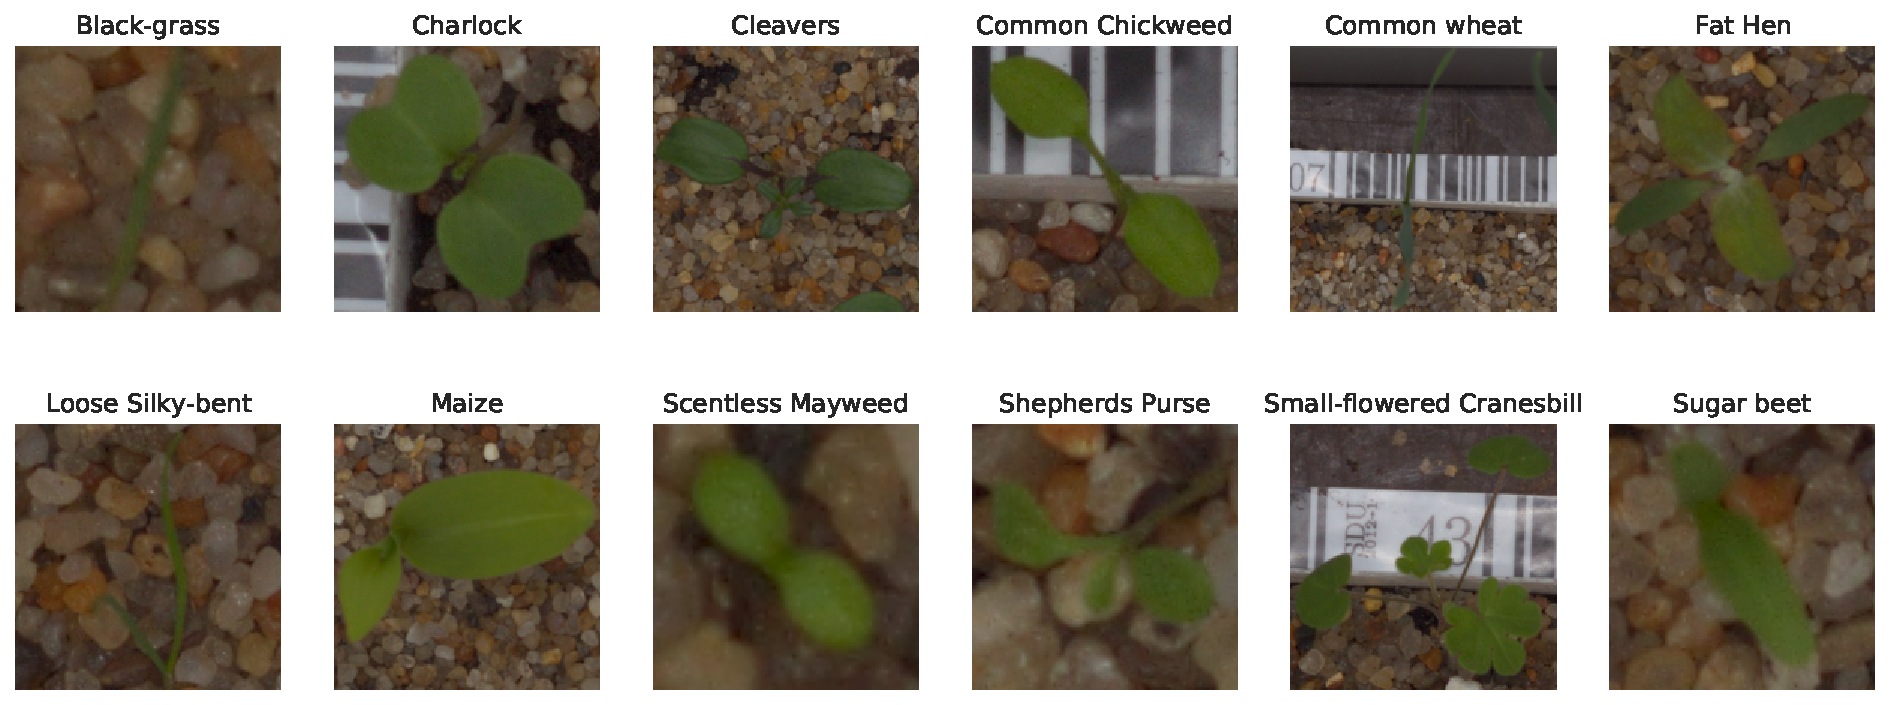
\includegraphics[width=1.0\linewidth]{samples_images.pdf}
			\end{center}
			\label{fig:samples}
		\end{figure}

		
	\end{itemize}
	
\end{frame}


\begin{frame}
	\frametitle{Tested methods}
	
	\begin{itemize}
		\item ResNet101 with ImageNet pretrained
		\item ResNeXt-101-32x8d - ImageNet pretrained
		\item ResNeXt-101-32x8d - Instagram  + ImageNet pretrained
		\item ResNeXt-101-32x16d - Instagram + ImageNet pretrained
		
		\begin{figure}[h]
			\begin{center}
				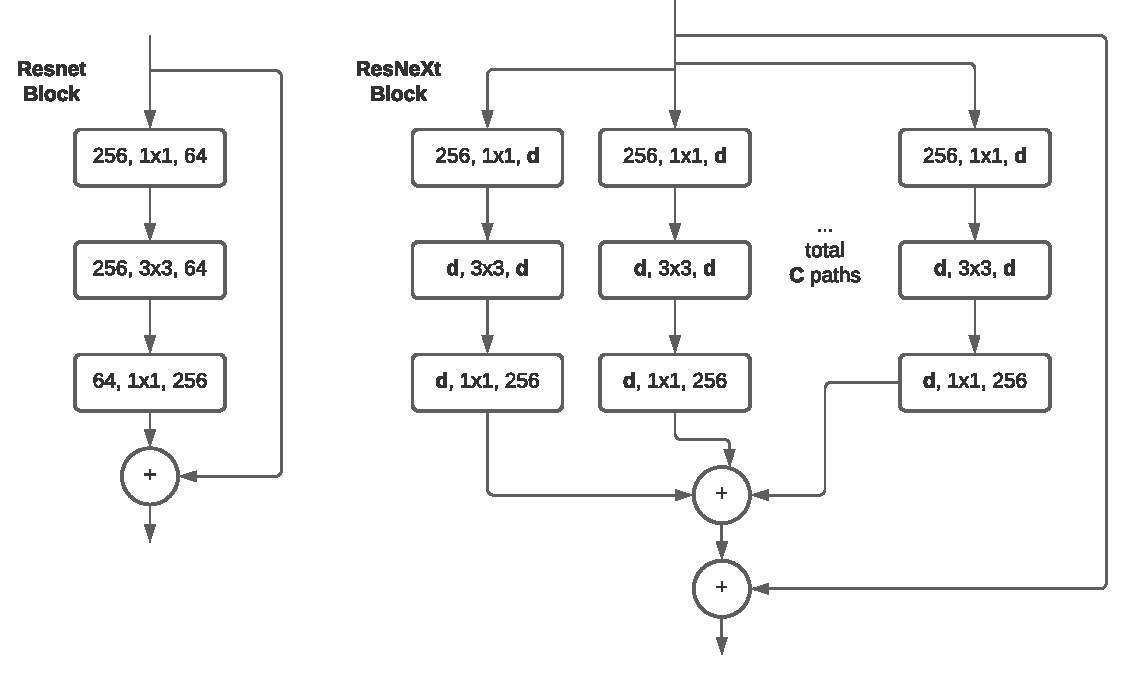
\includegraphics[width=1.0\linewidth]{resnet_resnext_block.pdf}
			\end{center}
			\label{fig:resnet}
			\end{figure}
		
		
	\end{itemize}
	
\end{frame}


\begin{frame}
	\frametitle{Training}
	
	\begin{itemize}
		\item Data augmentation: 
			\begin{itemize}
			\item Random Crop
			\item Random horizontal flip 
			\item Random resize
			\end{itemize}
		\item Training in two stages
		    \begin{itemize}
			\item 20 epochs training the last linear layer
			\item 20 epochs training the complete neural network
			\end{itemize}
		\item Learning rate decrease every 7 epochs
		
		
	\end{itemize}
	
\end{frame}

\begin{frame}
	\frametitle{Learning Rate tuning}
	

\begin{figure}[h]
	\begin{center}
		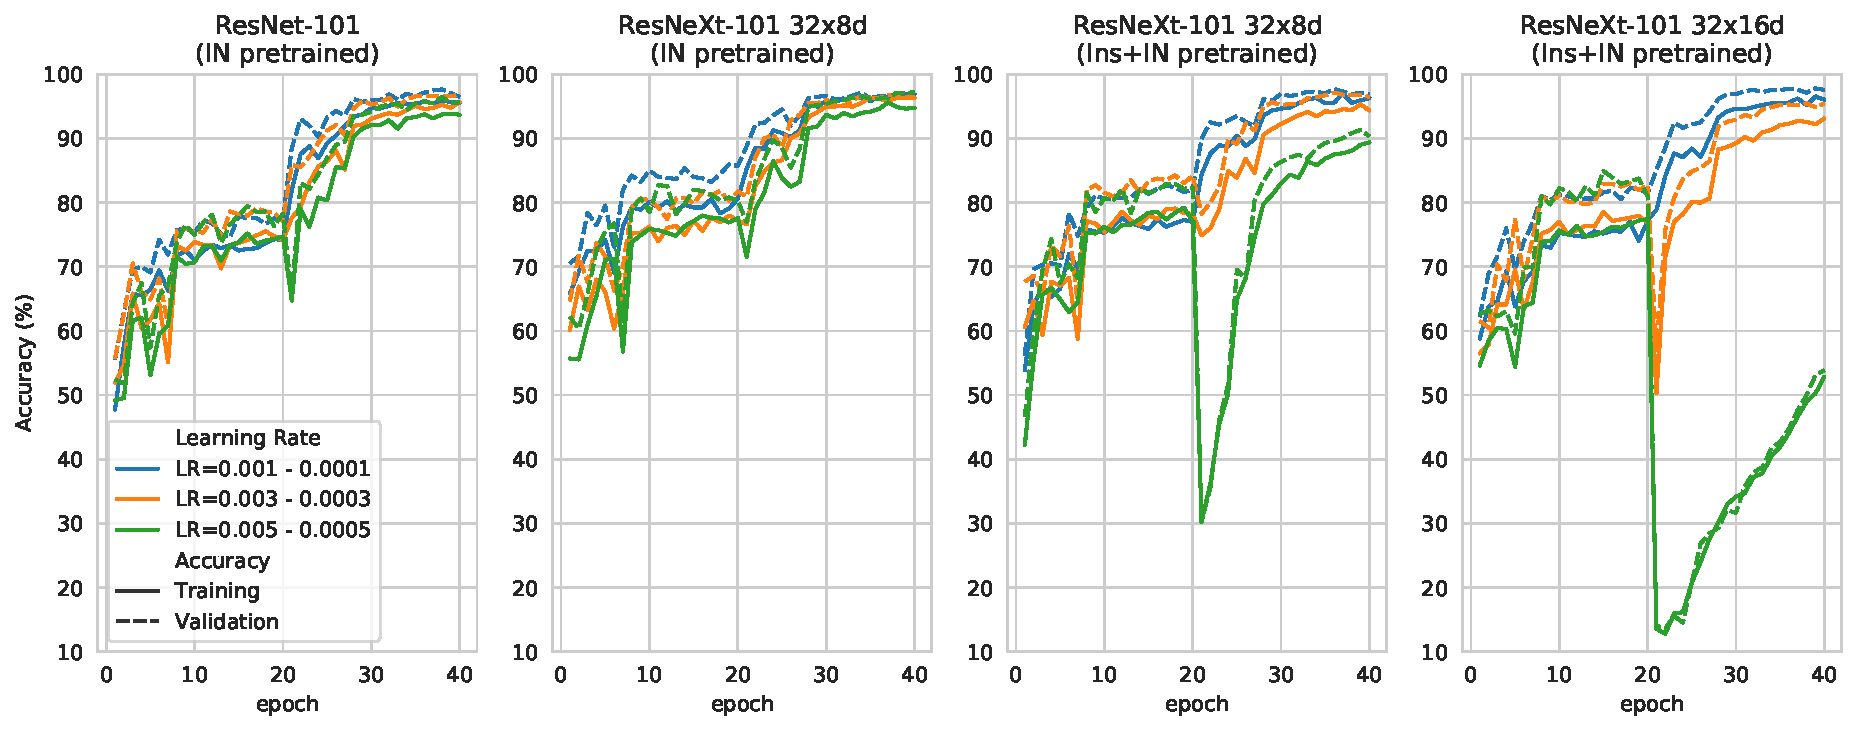
\includegraphics[width=0.75\linewidth]{lr_4models.pdf}
	\end{center}
	\label{fig:lr}
\end{figure}
.

\begin{figure}[h]
	\begin{center}
		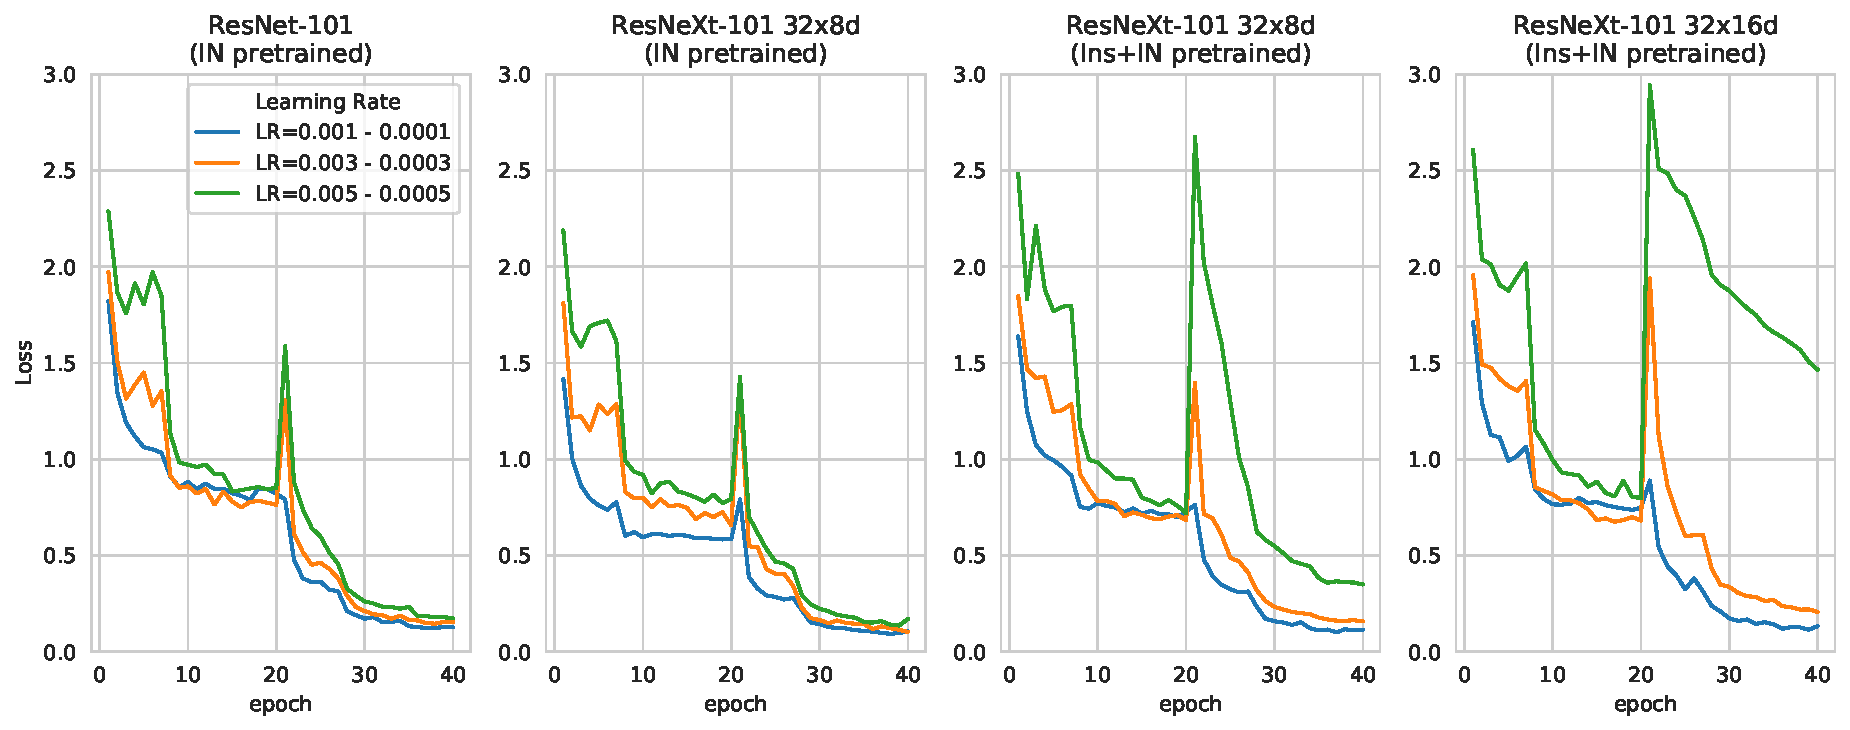
\includegraphics[width=0.75\linewidth]{loss_4models.pdf}
	\end{center}
\end{figure}

	
\end{frame}

\begin{frame}
	\frametitle{Validation data performance}
	
\begin{table}[h]
	\footnotesize
	\begin{center}
		\begin{tabular}{|p{3.4cm}|p{1.7cm}|p{1.7cm}|p{1.7cm}|p{1.7cm}|}
			\hline
			Class & ResNet-101 (IN Pretrained) & ResNeXt-101 32x8d (IN Pretrained) & ResNeXt-101 32x8d (Ins+IN Pretrained) & ResNeXt-101 32x16d (Ins+IN Pretrained)\\
			\hline\hline
			Black-grass &  \textcolor{red}{76.67\%} &\textcolor{red}{81.67\%}  & \textcolor{red}{76.67\%}  & \textcolor{red}{85.00\%}  \\
			Charlock & 100.00\% & 100.00\% & 100.00\% & 100.00\% \\
			Cleavers & 95.89\% & 97.26\% & 98.63\% & 100.00\%  \\
			Common Chickweed & 100.00\% & 98.51\% & 100.00\% & 99.25\%\\
			Common wheat & 96.43\%  & 98.21\% & 96.43\% & 92.86\%\\
			Fat Hen & 100.00\% & 99.21\% & 99.21\% & 99.21\% \\
			Loose Silky-bent & 95.83\% & 97.62\% & 92.26\% & 92.86\% \\
			Maize & 98.18\% & 100.00\% & 100.00\% & 100.00\% \\
			Scentless Mayweed & 97.71\% & 97.71\% & 97.71\% & 97.71\% \\
			Shepherds Purse & 89.83\% & 96.61\% & 94.92\% & 100.00\% \\
			Small-flowered Cranesbill & 100.00\% & 100.00\% & 98.46\% & 99.23\% \\
			Sugar beet & 98.02\% & 96.04\% & 99.01\% & 97.03\% \\
			\hline
			\textbf{Overall accuracy} & \textbf{96.80\%} & \textbf{97.47\%} & \textbf{96.63\%} & \textbf{97.14\%} \\
			\hline
		\end{tabular}
	\end{center}
	\label{table:val}
\end{table}

	
\end{frame}


\begin{frame}
	\frametitle{Validation data performance}
	
	\begin{figure}[h]
		\begin{center}
			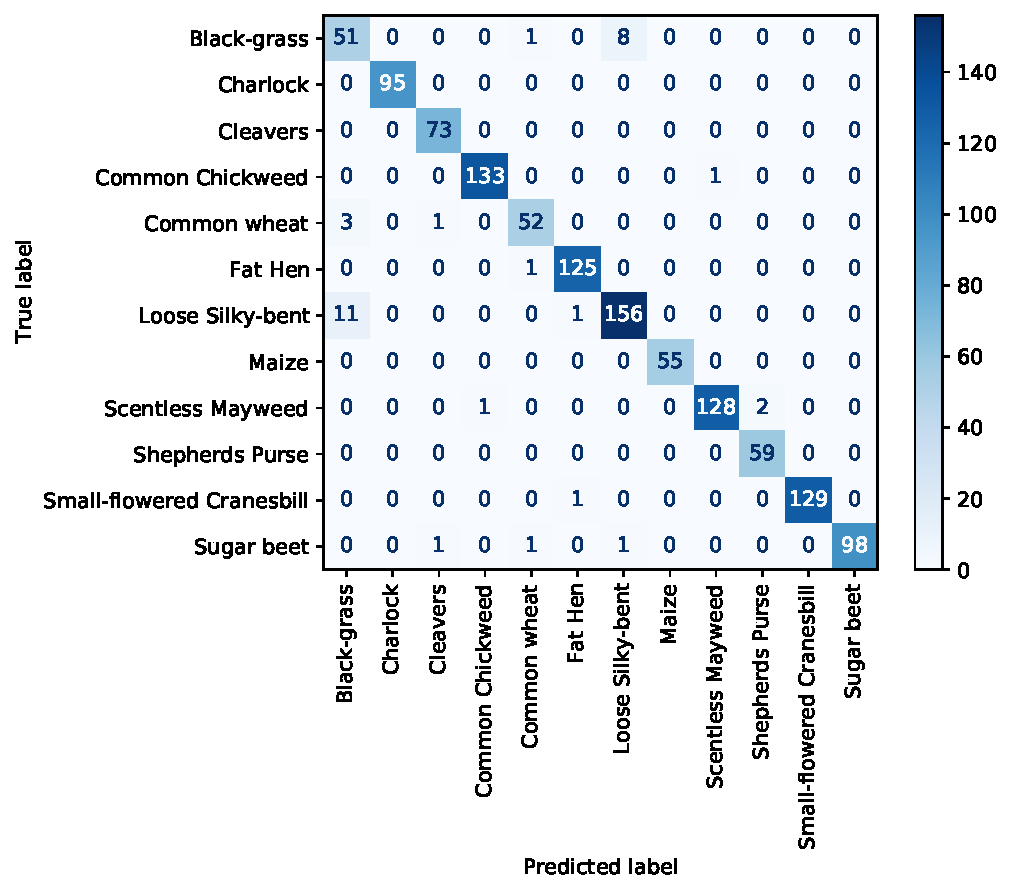
\includegraphics[width=0.78\linewidth]{confusion_matrix.pdf}
		\end{center}
		\label{fig:cm}
	\end{figure}
	
\end{frame}

\begin{frame}
	\frametitle{Test data: Kaggle submission}
	
\begin{table}[h]
	\footnotesize
	\begin{center}
		\begin{tabular}{|p{5cm}|p{2.8cm}|p{2.8cm}|}
			\hline
			Model & Mean F1 Score (Overall accuracy) & Simulated Leaderboard position\\
			\hline\hline
			Resnet-101 (IN Pretrained) & 0.97103 & 262/833 (31.45\%) \\
			ResneXt-101 32x8d (IN Pretrained) & \textbf{0.97858} & \textbf{149/833 (17.89\%)}  \\
			ResneXt-101 32x8d (Ins+IN Pretrained) & 0.97732 & 173/833 (20.77\%)   \\
			ResneXt-101 32x16d (Ins+IN Pretrained) & 0.97229 & 248/833 (29.77\%) \\
			\hline
		\end{tabular}
	\end{center}
	\label{table:test}
\end{table}

	\begin{figure}
	\centering
	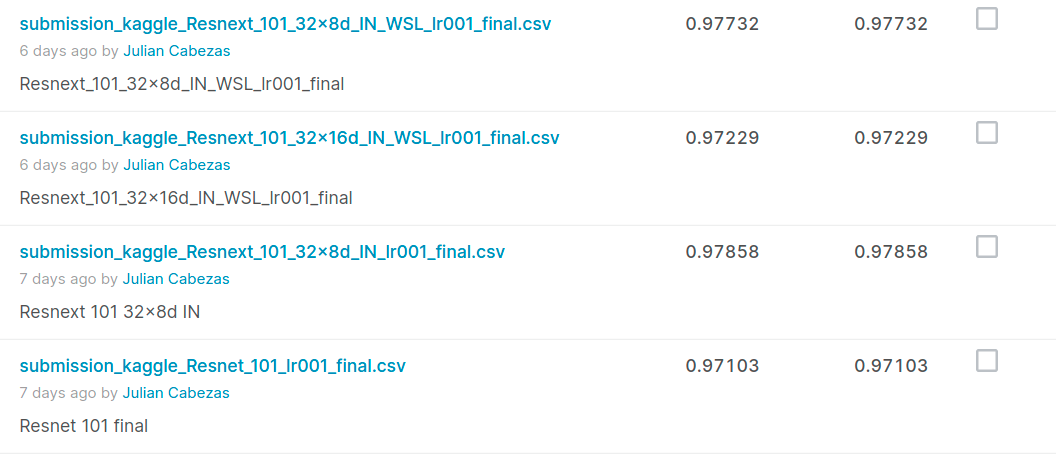
\includegraphics[width=0.7\linewidth]{Screenshot}
	\label{fig:screenshot001}
\end{figure}

Kaggle user: JulianCabezas
	
\end{frame}

\begin{frame}
	
	\frametitle{Conclusion}
	
	\begin{itemize}
		\item The pretraining using the Instagram data does not produce better results than the ImageNet pretraining in this case
		\item ResNeXt architecture slightly outperformed equivalent ResNet Neural networks 
		\item Pretrained models can produce competitive, accurate and time efficient predictions for plant seedling classification
	\end{itemize}
	
	
\end{frame}


\end{document}